\documentclass[a4paper, 12pt]{article}
\usepackage[left=2cm,text={17cm, 24cm},top=3cm]{geometry}
\usepackage[czech]{babel}
\usepackage[utf8]{inputenc}
\usepackage[IL2]{fontenc}
\usepackage{graphics}
\usepackage{url}
\usepackage{pgf}
\usepackage{tikz}
\usetikzlibrary{arrows,automata}
\usepackage{diagbox}
\usepackage{pdflscape}
\usepackage{etoolbox}
\patchcmd{\thebibliography}{\section*{\refname}}{}{}{}
\pagenumbering{arabic}
\providecommand{\uv}[1]{\quotedblbase #1\textquotedblleft}
\interlinepenalty 10000 %nezalamovat odstavce

\begin{document}
\begin{titlepage}

\begin{center}
\fontsize{25}{20}\selectfont{\textsc{Vysoké učení technické v~Brně}}\\
\vspace{\stretch{0.0075}}
\fontsize{21}{0}\textsc{\selectfont{Fakulta informačních technologií}}\\
\vspace{\stretch{0.15}}


\begin{figure}[ht]
    \begin{center}
        \scalebox{0.20}{\includegraphics{fit.png}}
    \end{center}
\end{figure}

\vspace{\stretch{0.2}}
\Large{Dokumentace k projektu do předmětů IFJ}\\
\LARGE{Implementace interpretu jazyka IFJ18}\\
\vspace{\stretch{0.618}}
Tým 61, varianta I \\
\vspace{\stretch{0.618}}
\end{center}

\begin{large}
{\Large
\begin{tabular}{llll}
  \\[-0.5em]
  Vedoucí:  & David Bulawa        & \texttt{xbulaw01} \ & 25 \\
  Členové:  & Jakub Dolejší       & \texttt{xdolej09} \ & 25 \\
            & František Policar   & \texttt{xpolic04} \ & 25 \\
            & Tomáš Svěrák        & \texttt{xsvera04} \ & 25 \\ \medskip \\
\end{tabular}
}
\end{large}

\end{titlepage}

%*******************************************************************************
%                   Obsah
%*******************************************************************************
\tableofcontents
\newpage
%*******************************************************************************
%                   Úvod
%*******************************************************************************
\section{Úvod} \label{uvod}

Dokumentace popisuje implementaci překladače imperativního jazyka IFJ18, který je podmnožinou jazyka Ruby2.0. Níže najdete popis průběhu vývoje, použité algoritmy a datové struktury. 

\section{Práce v~týmu} \label{team}

\subsection{Rozdělení práce na jednotlivých částech projektu}
\begin{itemize}
                \item David Bulawa -- Rekurzivní sestup, generování, návrh LL-gramatiky
                \item Jakub Dolejší -- Lexikální analyzátor, tabulka symbolů, generování, precedenční analýza
                \item František Policar -- Dokumentace, prezentace, konečný automat, rekurzivní sestup 
                \item Tomáš Svěrák  -- Lexikální analyzátor, generování, precedenční analýza, návrh zásobníků 
                
\end{itemize}

\subsection{Průběh vývoje}

Na projektu se podílel čtyřčlenný tým, bylo tedy třeba dobře rozdělit a rozvrhnout práci. Po domluvě jsme využili verzovací systém {\bf Subversion} na serveru github.com. Problémy a postup řešení projektu jsme konzultovali alespoň dvakrát týdně. Na začátku měl každý přidělenou část projektu, kterou měl zpracovat (vyjma složitějších částí, které jsme dělali společně), a následně jsme jednotlivé moduly začali propojovat mezi sebou.

\newpage

\section{Implementace interpretu jazyka IFJ18} \label{implementace}
\subsection{Lexikální analýza} \label{lexer}

Lexikální analýza je činnost, kterou provádí tzv. lexikální analyzátor (SCANNER). 
Lexikální analyzátor rozdělí vstupní posloupnost znaků na lexémy - např. identifikátory, operátory. 
Tyto lexémy jsou reprezentovány ve formě tokenů, ty jsou poskytnuty ke zpracování syntaktickému analyzátoru (PARSERU). Lexikální analyzátor jsme implementovali pomocí deterministického konečného automatu (dále DKA). Jediná výjimka je v případě přechodu do blokového komentáře, kde determinismus nebylo možné zachovat (implementačně ošetřeno boolovskou proměnnou, která značí nový řádek). Následně DKA zjistí typ tokenu, do kterého uloží jeho typ, a v případě identifikátoru/čísla i jeho hodnotu(atribut). Pokud DKA došel do koncového stavu, odesílá token syntaktické analýze a vrací se zpět do počátečního stavu. V jiném případě vrací lexikální chybu. 

\subsection{Syntaktická analýza} \label{parser}

Syntaktický analyzátor (PARSER) je jádro celého překladače. Na základě pravidel sestavených dle LL – gramatiky (Příloha 4.A a 4.B) jsme vytvořili funkce pro rekurzivní sestup, který je kombinovaný s precedenční analýzou pro výpočet výrazů. SA žádá LA o tokeny, které následně zpracovává. Rekurzivní sestup je implementován dvouprůchodově s využitím bufferu. První průchod se skládá z částečné kontroly syntaxe a naplnění tabulky symbolů. Druhý průchod kontroluje zbylou syntaxi, sémantiku a generuje cílový kód.     

\subsection{Precedenční analýza} \label{prec_analyza}

Precedenční analýza je separátní část SA, která se stará o zpracování výrazů. Nejprve jsme si vytvořili seznam redukčních pravidel a precedenční tabulku dle priority operátorů. Tabulka byla implementována pomocí dvourozměrného pole ENUMů, kde sloupce vyjadřovaly aktuální token na vstupu a řádky symbol na zásobníku. Abychom v tabulce mohli řádně indexovat, převedli jsme vstupní token automaticky na stejný datový typ jako symboly na zásobníku. Dále jsme si vytvořili funkce pro ověření pravidel a následnou redukci v případě správně nalezeného pravidla. Hlavní tělo precedenční analýzy jsme implementovali dle algoritmu z přednášky. Ten spočívá v nalezení indexu v precedenční tabulce a jeho vyhodnocení dle předepsaných pravidel. Zde jsme provedli změny ohledně práci s tokeny; namísto žádání LA o další token si pouze posuneme ukazatel na další prvek v bufferu, do kterého si tokenu ukládáme. \\
Vzhledem k tomu, že jazyk IFJ18 je dynamicky typovaný, tak jsme sémantické kontroly výrazů nemohli provádět zde, ale až na úrovni generování.

\subsection{Generování} \label{gener}

Po úspěšném dokončení lexikální analýzy a prvním průchodu syntaktické analýzy se začíná generovat cílový kód. Na standardní výstup generujeme jednotlivé instrukce. Opět zde probíhá předávání řízení mezi rekurzivním sestupem a precedenční analýzou. Provádí se zde typové kontroly a konverze při výpočtu výrazů. Instrukce se generují přímo na standardní výstup.  


%Následující dva řádky obsahují instrukce CREATEFRAME\footnote{CREATEFRAME - Vytvoří nový dočasný rámec} a PUSHFRAME\footnote{PUSHFRAME - Přesune dočasný rámec na zásobník rámců}. 

%\subsection{Zpracování jazykových konstrukcí, výrazů a volání funkcí} \label{zp_ja_kon}

%Syntaktická analýza je implementována rekurzivním sestupem, který řídí naše LL-gramatika (příloha 4.B). 
%V tomto případě neterminály představují tokeny, které se přenášejí z lexikálního analyzátoru.

\newpage

\subsection{Použité algoritmy a datové struktury}

\subsubsection{Buffer}

Ačkoliv jsme měli využívat LL(1) gramatiku, tak v několika případech bylo nutno se podívat o více než jeden token dopředu. Z tohoto důvodu jsme implementovali buffer, do kterého jsme tokeny nahrávali. Pokud se tedy SA potřebovala podívat o více tokenů dopředu a následně je vrátit, tak jednoduše posunula ukazatel na aktuální prvek v bufferu dozadu.

\subsubsection{BVS}

Vzhledem k tomu, že naše skupina má variantu 1, tak jsme tabulku symbolů implementovali pomocí binárního stromu. Každá položka (uzel) BVS v sobě obsahuje vyjma ukazatele na levý a pravý podstrom a ukazatele na pod tabulku, informace, zda se jedná o proměnnou či funkci, či byla definovaná a počet parametrů v případě funkce.

\subsubsection{Dynamický string}

Vzhledem k tomu, že v jazyce C neexistuje typ string, tak jsme byli nuceni si vytvořit vlastní datový typ pro řetězec, abychom mohli provádět kupříkladu konkatenaci. V tomto případě jsme se inspirovali soubory 	{\bf str.c} a {\bf str.h} z ukázkového interpretu dostupného na stránkách předmětu.

\subsubsection{Zásobník}

Zásobník (STACK) je dynamická datová struktura používaná pro dočasné ukládání dat. 
Má uplatnění pro precedenční syntaktickou analýzu. Nejvíce se využívá při převodu infixového zápisu na postfixový.

\subsubsection{Postfix}

Pro vyčíslení výrazů a vygenerování cílového kódu u precedenční syntaktické analýzy jsme použili postfixový zápis. Ten značně zjednodušil práci s mezivýsledky, kdy jsme si nemuseli vytvářet pomocné proměnné. 

\section{Závěr} \label{zaver}

Už ze začátku bylo jasné, že se bude jednat o zatím největší projekt, co jsme zde měli, proto jsme ho nechtěli podcenit. V průběhu práce na projektu jsme se potýkali s řadou problémů, které povětšinou vyřešilo diskuzní fórum, stránky z přednášek, či vzájemné diskuze.

\newpage

%\begin{landscape}
\section{Přílohy} \label{prilohy}

\renewcommand\thesubsection{\thesection.\Alph{subsection}}
\subsection{Diagram konečného automatu lexikální analýzy} 

\begin{figure}[ht]
    \begin{center}
        \scalebox{0.3}{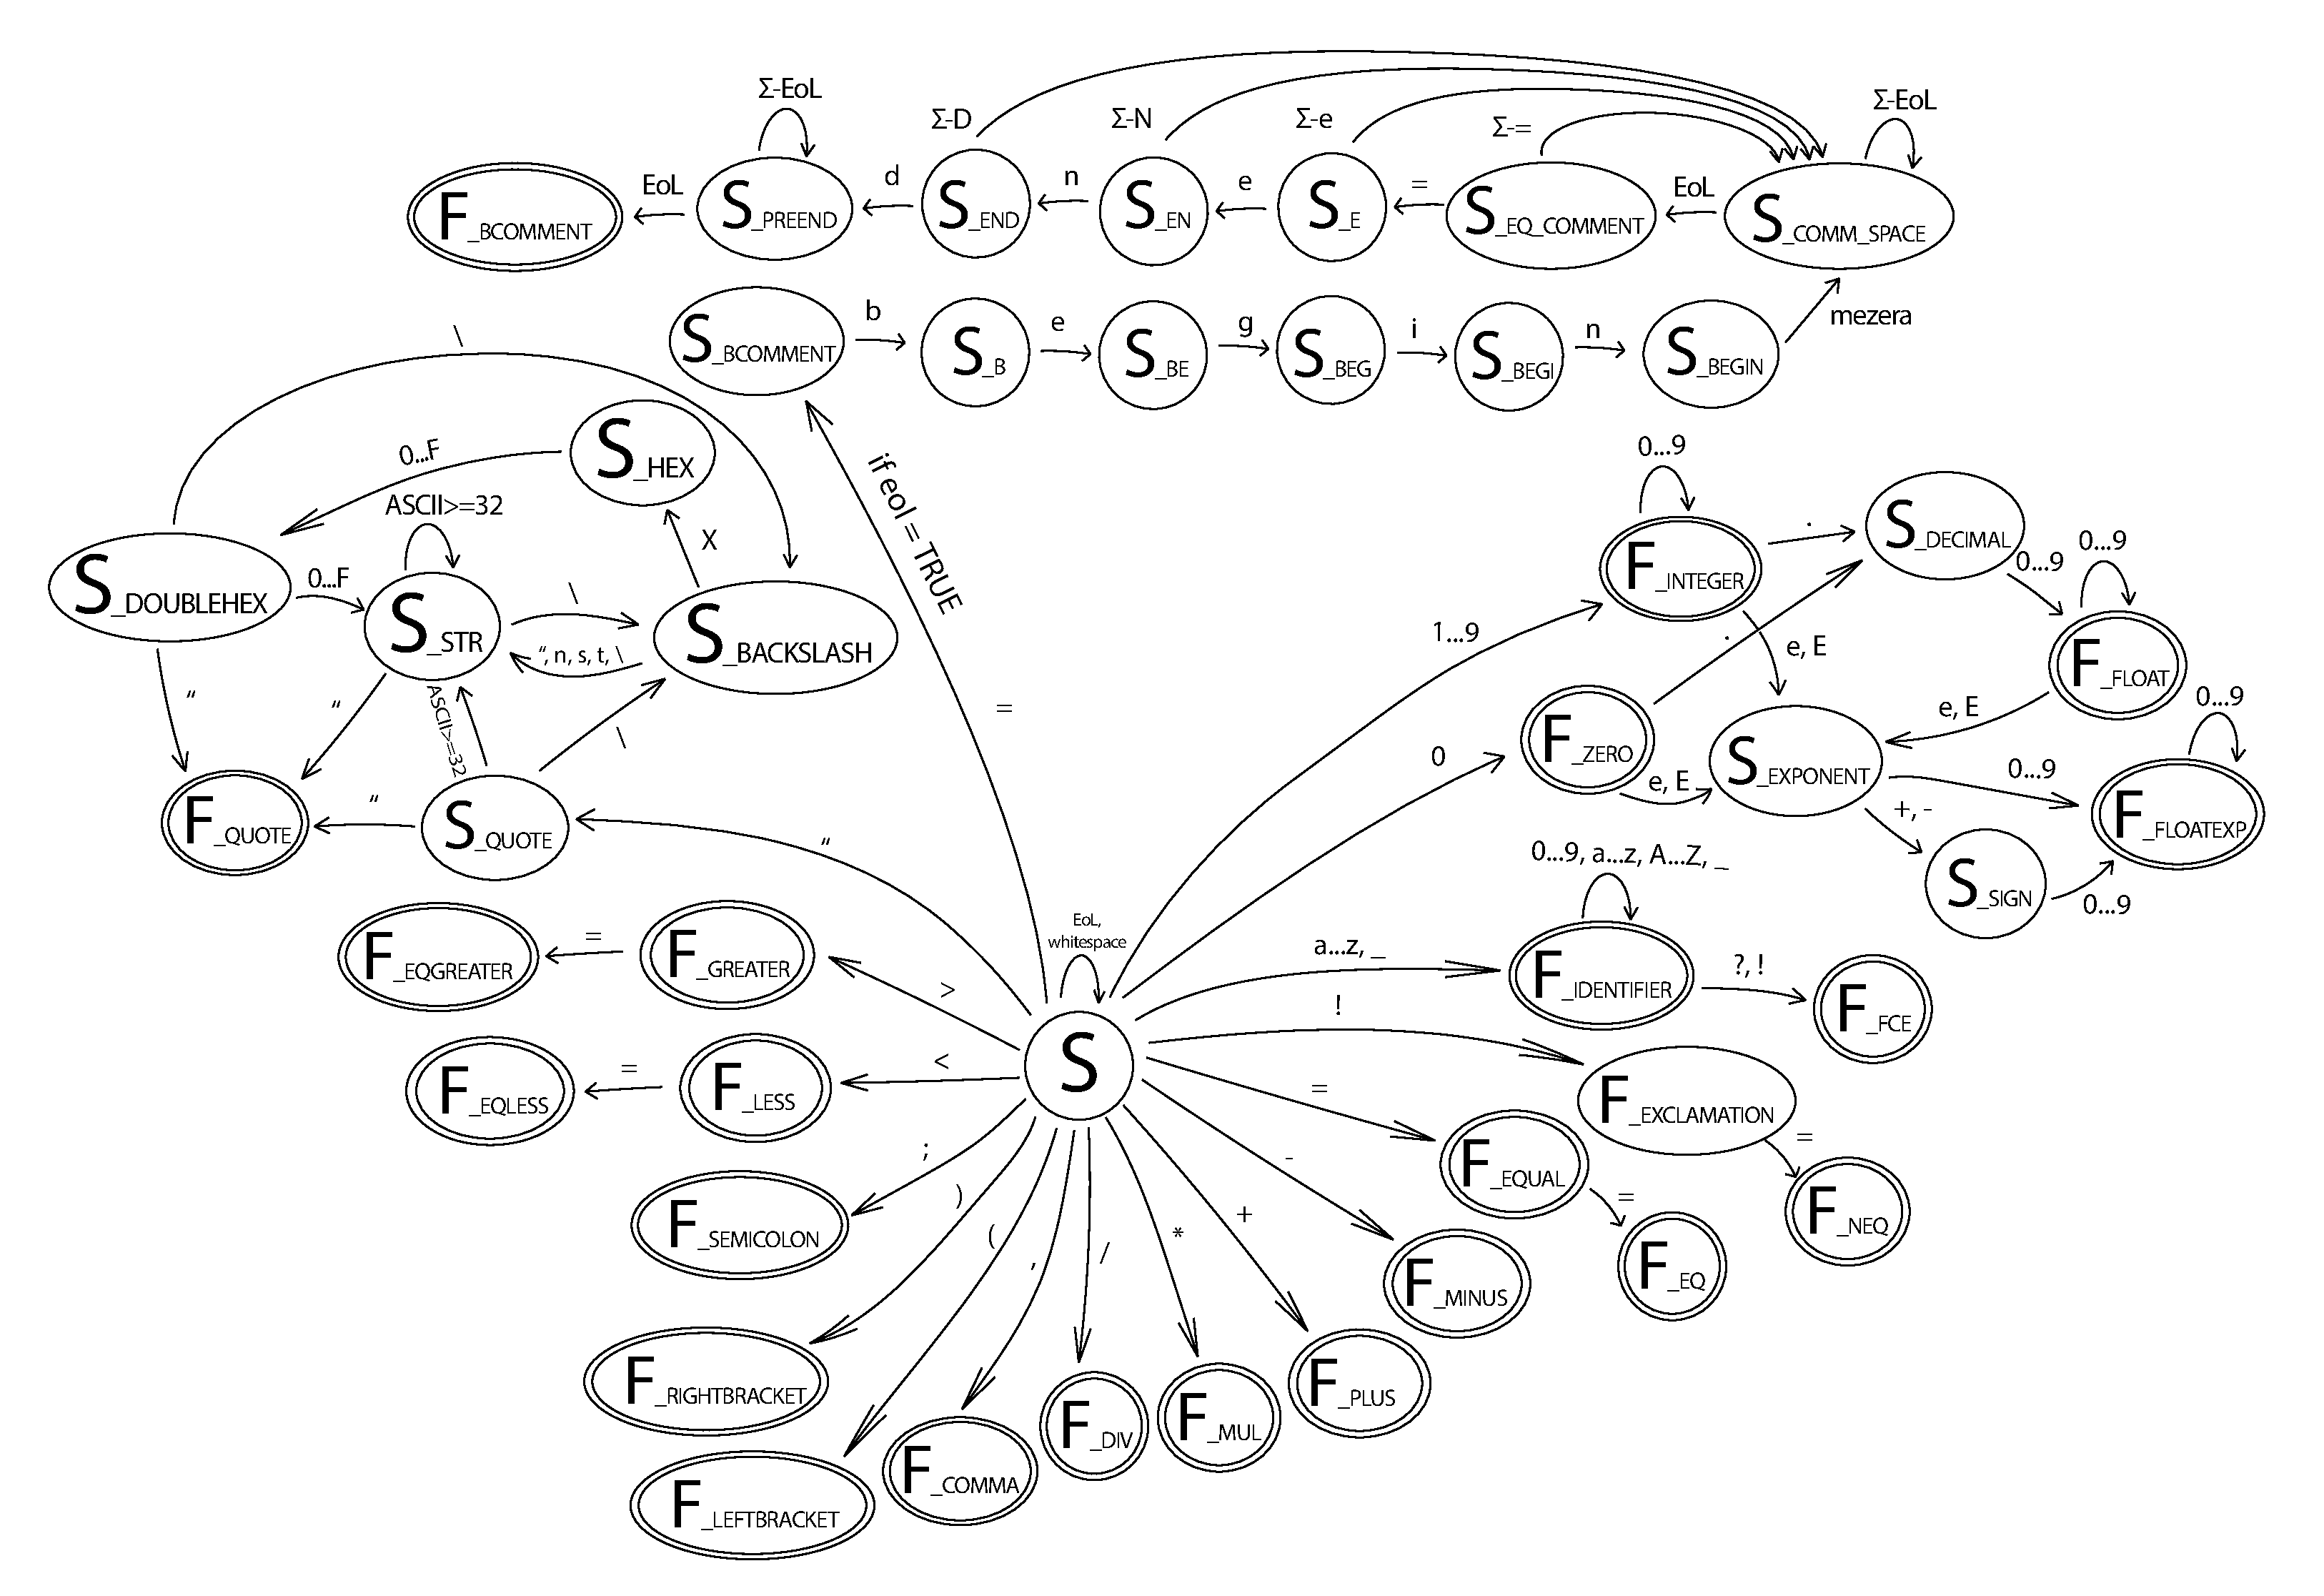
\includegraphics{scanner_gra.pdf}}
    \end{center}
\end{figure}

%\end{landscape}

\newpage

\subsection{LL-gramatika} \label{subsec:llgram}
\begin{verbatim}
1. PROG -> SEC END_ROW PROG
2. PROG -> eol PROG
3. PROG -> ''
4. PROG -> eof
5. PROG -> bcomment PROG
6. END_ROW  -> eol
7. END_ROW  -> eof
8. SEC -> identifier eq FCE_EXPR
9. SEC -> while EXPR do eol PROG end
10. SEC -> if EXPR then eol PROG else eol PROG end
11. SEC -> def identifier lbracket PARAMS rbracket eol PROG end
12. PARAMS -> ''
13. PARAMS -> identifier PARAM_LIST
14. PARAM_LIST -> ''
15. PARAM_LIST -> comma identifier PARAM_LIST
16. CALL_PARAMS -> ''
17. CALL_PARAMS -> ITEM CALL_PARAM_LIST 
18. CALL_PARAM_LIST -> ''
19. CALL_PARAM_LIST -> comma ITEM CALL_PARAM_LIST 
20. FCE_EXPR -> EXPR
21. FCE_EXPR -> FCE
22. BR_OR_NOT -> lbracket CALL_PARAMS rbracket 
23. BR_OR_NOT -> CALL_PARAMS 
24. FCE -> identifier BR_OR_NOT
25. ITEM -> integer
26. ITEM -> float
27. ITEM -> string
28. ITEM -> nil
29. ITEM -> identifier
30. EXPR -> ''

\end{verbatim}

\newpage

%\begin{landscape}
%\begin{figure}[ht]
    \begin{center}
        \scalebox{0.95}{\includegraphics{LL_table_nume.pdf}}
    \end{center}
%\end{figure}
%\end{landscape}  

\newpage

\subsection{Precedenční tabulka} \label{subsec:precetable}


\begin{figure}[ht]
    \begin{center}
        \scalebox{0.5}{\includegraphics{Precedencni_tabulka.pdf}}
    \end{center}
\end{figure}               

\end{document}
